\documentclass[presentation,aspectratio=169]{beamer}
\usepackage[utf8]{inputenc}
\usepackage[T1]{fontenc}
\usepackage{graphicx}
\graphicspath{{./graphics/}}
\usepackage[ngerman]{babel}
\usepackage{longtable,capt-of,fvextra,csquotes}
\MakeOuterQuote{"}
\usepackage{wrapfig,rotating}
\usepackage[normalem]{ulem}
\usepackage{amsmath,amssymb}
\usepackage{hyperref}
\usepackage{listings,minted}
\usepackage[duration=20]{pdfpc}
\usetheme{metropolis}
\author{Julius Freudenberger}
\date{Cyberweek Sommersemester 2025}
\title{WYSIWYAF with \LaTeX}
\subtitle{Einstieg in Wissenschaftliche Arbeiten mit \LaTeX}
\mode<presentation>{\usetheme{metropolis}}
\mode<beamer|handout>{\metroset{sectionpage=progressbar}}
\mode<beamer|handout>{\metroset{subsectionpage=progressbar}}
\mode<beamer|handout>{\metroset{progressbar=frametitle}}
\mode<beamer|handout>{\metroset{block=fill}}
\institute[Hochschule Esslingen]{Hochschule Esslingen}
\hypersetup{
  pdfauthor={Julius Freudenberger},
  pdftitle={WYSIWYAF with LaTeX},
  pdfkeywords={},
  pdfsubject={},
  pdflang={German},
  colorlinks,
  linkcolor=black,
  citecolor=black,
  filecolor=black,
  urlcolor=blue
}
\usepackage{biblatex}

\begin{document}

\maketitle

\begin{frame}[fragile]{Bevor wir beginnen: Was brauche ich?}
  \begin{itemize}
    \item \LaTeX-Distribution: \TeX{}Live oder Mik\TeX{}
      \begin{itemize}
        \item Windows: \href{https://miktex.org/}{https://miktex.org/}
        \item Mac: \href{https://tug.org/mactex/}{https://tug.org/mactex/}
        \item Linux: Installation über den Paketmanager
          \begin{itemize}
            \item deb: \verb|texlive-base|, rpm: \verb|texlive texlive-latex|
            \item Arch Linux: \verb|texlive-core|
            \item NixOS: \verb|nixpkgs.texliveBasic|
          \end{itemize}
        \item Docker: \verb|texlive/texlive|
      \end{itemize}
    \item Texteditor
      \begin{itemize}
        \item \href{https://code.visualstudio.com/}{VSCode} mit \href{https://marketplace.visualstudio.com/items?itemName=James-Yu.latex-workshop}{\LaTeX-Workshop}, \href{https://www.vim.org/}{vim} mit \href{https://github.com/lervag/vimtex}{vimtex}
        \item \href{https://www.xm1math.net/texmaker/index.html}{\TeX{}Maker}
      \end{itemize}
    \item Alternativ: Online-Editoren
      \begin{itemize}
        \item Overleaf (\href{https://www.overleaf.com}{https://www.overleaf.com}, Registrierung erforderlich)
        \item \TeX{}Viewer (\href{https://texviewer.herokuapp.com}{https://texviewer.herokuapp.com}, direkt nutzbar)
      \end{itemize}
  \end{itemize}
\end{frame}

\begin{frame}{Über mich}
  \textbf{B.\,Eng. Julius Freudenberger}
  \begin{itemize}
    \item 2000 geboren
    \item 2016 erste Kontakte mit \LaTeX
    \item 2019 -- 2023 Bachelorstudium an der Hochschule Esslingen
    \item 2023 -- 2026(?) Masterstudium an der Hochschule Karlsruhe
    \item nebenbei Werkstudent
  \end{itemize}
\end{frame}

\begin{frame}{Wer seid ihr?}
  \begin{itemize}
    \item Name
    \item Fakultät? Was macht ihr da?
    \item Schon von \LaTeX{} gehört oder etwas damit gemacht?
    \item Was stört dich am meisten an traditionellen Textverarbeitungsprogrammen?
    \item Nächste (wissenschaftliche) Arbeit, die du vielleicht mit \LaTeX{} schreiben möchtest?
  \end{itemize}
\end{frame}

\begin{frame}{Materialien für den Kurs}
  \begin{itemize}
    \item Dieser Foliensatz
    \item Kleine Vorlagen zum Mitmachen
    \item Dokumente, die wir im Laufe des Kurses erstellen
      \bigskip
    \item wird alles im geteilten Ordner hochgeladen
  \end{itemize}
\end{frame}

\begin{frame}{Inhalt}
  \tableofcontents
\end{frame}

\section{\LaTeX{} -- die Theorie}

\begin{frame}{Was ist \LaTeX?}
  \pdfpcnote{ - Entwicklung seit Anfang der 1980er
  - What you see is what you get --> What you see is what you asked for}
  \begin{itemize}
    \item Textsatzsystem
    \item setzt vorgegebenen Text und weitere Anweisungen automatisch
    \item versucht automatisch bestmögliches Layout
    \item kein WYSIWYG, sondern WYSIWYAF
    \item Quellcode wird "kompiliert"
    \item Dokument wird als PDF, PS, DVI oder sogar HTML ausgegeben
  \end{itemize}
\end{frame}

\begin{frame}{Warum \LaTeX?}
  \pdfpcnote{ Vergleich zu Word
    - schöner Blocksatz, bestmögliche Zeilenumbrüche und Worttrennungen
    - Inhaltsverzeichnis und Verzeichnisse für Abbildungen, Stichworte, Abkürzungen und Literatur
    - Abbildungen und weitere Referenzelemente werden automatisch an der bestmöglichen Stelle eingefügt
  - Deutlich mehr Automatisierungen als bei Word, "Layoutarbeit" am Ende einer Arbeit deutlich geringer}
  \begin{columns}[t]
    \column{.4\textwidth}
      \begin{itemize}
        \item Automatischer Textsatz
        \item Automatische Referenzen
        \item Automatisches Layout
      \end{itemize}
    \column{.5\textwidth}
      \begin{itemize}
        \item Keine große Layoutarbeit am Ende
        \item Kein Ruinieren des Dokuments beim Verschieben eines Bildes
        \item Das Dokument "sieht einfach schön aus"
      \end{itemize}
  \end{columns}
  \begin{center}
    Wenn man einmal \LaTeX{} gelernt hat, ist das Layouten von wissenschaftlichen Arbeiten deutlich einfacher.
  \end{center}
\end{frame}

\begin{frame}{Wie sieht \LaTeX-Code aus?}
  \pdfpcnote{
    - Befehle werden mit \ angegeben
    - Parameter mit {}
    - Einrückung hilft bei Lesbarkeit, ist nicht notwendig
    - Beginn und Ende
    - normaler Text
  }
  \inputminted{latex}{codebeispiele/beispiel.tex}
\end{frame}

\begin{frame}{Grundlegender Aufbau}
  \pdfpcnote{
    - Dokumentenklasse (book, article, report)
    - Präambel
    - Metadaten (Titel, Autor, Datum)
    - Zusätzliche Pakete -> großes Ökosystem mit Paketen für alles was man sich vorstellen kann
    - Einstellungen
    - Eigentliches Dokument
  }
  \inputminted{latex}{codebeispiele/aufbau.tex}
\end{frame}

\begin{frame}[fragile]{Präambel}
  \begin{itemize}
    \item Dokumentenklasse
      \begin{itemize}
        \item \verb|scrartcl| für Artikel und kürzere Arbeiten
        \item \verb|scrbook| für Bücher oder Thesen
        \item \verb|letter| oder \verb|dinletter| für Briefe und Anschreiben
        \item Klassen mit \verb|scr| sind KOMA-Klassen.
          \begin{itemize}
            \item modern
            \item viele gute Standardeinstellungen
          \end{itemize}
      \end{itemize}
    \item Pakete
    \item Einstellungen
  \end{itemize}
\end{frame}

\section{Direkt ausprobieren und mitmachen}

\begin{frame}[fragile]{Vorlage herunterladen}
  \begin{itemize}
    \item \href{https://www2.hs-esslingen.de/~jufrit00/latex/}{https://www2.hs-esslingen.de/\textasciitilde{}jufrit00/latex/}
    \item \href{https://gitlab.hs-esslingen.de/jufrit00/latex-workshop}{https://gitlab.hs-esslingen.de/jufrit00/latex-workshop}
    \item \href{https://github.com/JuliusFreudenberger/latex-workshop}{https://github.com/JuliusFreudenberger/latex-workshop}
      \bigskip
    \item Vorlage befindet sich im Ordner \verb|codebeispiele/vorlage.tex|
    \item diese am besten in einen neuen leeren Ordner kopieren
  \end{itemize}
\end{frame}

\begin{frame}[fragile]{Projekt kompilieren}
  \begin{itemize}
    \item Im Projektverzeichnis \verb|pdflatex file.tex|
    \item automatisierter mit \verb|latexmk -pdf file.tex|
    \item In \TeX{}Maker "Schnelles Übersetzen"
    \item mittels Docker und Docker Compose (Anleitung im Git Repo)
    \item Outputfile \verb|file.pdf| als PDF-Datei im gleichen Verzeichnis
  \end{itemize}
\end{frame}

\begin{frame}[fragile]{Erste eigene Änderungen}
  \pdfpcnote{
    - Stärke von LaTeX: Änderungen wirken sich konsistent auf das gesamte Dokument aus.
    - Keine manuelle Anpassung an mehreren Stellen nötig.
    - Hervorhebung hängt von Dokumenttyp und Einstellungen ab. Standard kursiv
    - Niedrigste Stufe: subsubsection
    - Bei Text am Besten ein Satz in eine Zeile.
  }
  \begin{itemize}
    \item Eigener Text, Absätze
    \item Textformatierung: \textbf{fett} und \textit{kursiv} mit \verb|\textbf{fett}|, \verb|\textit{kursiv}|
    \item \emph{Hervorhebung} im Text: \verb|\emph{hervorgehoben}|
    \item Eigene Abschnitte mit \verb|\section{} und \subsection{}|
    \item In Büchern zusätzlich \verb|\chapter|
    \item Metadaten ändern
      \begin{itemize}
        \item Titel des Dokuments ändern mit \verb|\title{}|
        \item Eigener Name als Autor mit \verb|\author{}|
        \item Anzeigen dieser Metadaten mit \verb|\maketitle|
      \end{itemize}
  \end{itemize}
\end{frame}

\maketitle

\section{Text, Inhalt und Struktur}

\begin{frame}[fragile]{Anführungszeichen}
  \begin{itemize}
    \item Standardmäßig wird ein \verb|"| direkt als solches gesetzt
    \item deutsche Anführungszeichen können mit den Befehlen \verb|\glqq{}| und \verb|\grqq{}| gesetzt werden
    \item mit dem Paket \verb|csquotes| können \verb|"| als sprachlich richtige Anführungszeichen angezeigt
      \begin{itemize}
        \item abhängig von der Spracheinstellung in \verb|babel|
      \end{itemize}
    \inputminted{latex}{codebeispiele/quotation.tex}
  \end{itemize}
\end{frame}

\begin{frame}[fragile]{Umgebungen}
  \begin{itemize}
    \item kennzeichnen besondere Bereiche im Dokument
    \item beginnen mit \verb|\begin{}| und enden mit \verb|\end{}|
    \item können verschachtelt werden, aber nicht geschnitten
    \item Aufzählungen \verb|enumerate| (nummeriert) und \verb|itemize| (unnummeriert)
  \end{itemize}
  \begin{columns}[t]
    \begin{column}{.3\textwidth}
      \centering
      \begin{minted}{latex}
\begin{itemize}
  \item Erster Punkt
  \item Zweiter Punkt
\end{itemize}
      \end{minted}
    \end{column}
    \begin{column}{.5\textwidth}
      \centering
      \begin{minted}{latex}
\begin{itemize}
  \item Erster Punkt
  \begin{enumerate}
    \item Anderer Punkt
  \end{itemize} % Das geht nicht
  \item Weiterer Punkt
\end{enumerate}
      \end{minted}
    \end{column}
  \end{columns}
\end{frame}

\begin{frame}[fragile]{Wichtige besondere Zeichen}
  \begin{tabular}{c|c|c}
    Schrägstrich                                  & \textbackslash   & \verb|\textbackslash| \\
    \hline
    Tilde                                         & \textasciitilde  & \verb|\textasciitilde| \\
    \hline
    geschütztes Leerzeichen (ohne Zeilenumbruch)  & ~                & \verb|~| \\
    \hline
    schmales geschütztes Leerzeichen              & z.\,B.           & \verb|z.\,B.| \\
    \hline
    Gedankenstrich (Halbgeviertstrich)            & --               & \verb|--| \\
    \hline
    Geviertstrich                                 & ---              & \verb|---|
  \end{tabular}
\end{frame}

\subsection{Verweise}

\begin{frame}{Verweise -- Was wollen wir?}
  \begin{itemize}
    \item Referenzieren von Abbildungen, Tabellen, Codezeilen, etc.
    \item automatische Nummerierung
    \item kein manuelles Nummerieren, Aktualisieren und Überprüfen
    \item automatische Verzeichnisse
  \end{itemize}
\end{frame}

\begin{frame}[fragile]{Verweise}
  \pdfpcnote{ - Label können frei wählbaren Namen bekommen
    - System ist dennoch hilfreich (fig:<name>, tab:<name>)
    - Wenn sich Seiten verschieben oder die Abbildung verschoben wird, aktualisieren sich automatisch alle Verweise und das dazugehörige Verzeichnis
    - erster Durchlauf: Anlegen einer Liste aller Verweise; zweiter Durchlauf: Einarbeiten aller gefunden labels
  }
  \begin{itemize}
    \item Label setzen: \verb|\label{<name>}|
    \item Abschnitt referenzieren: \verb|\ref{<name>}|
    \item Seite referenzieren: \verb|\pageref{<name>}|
    \item Referenz nutzt immer aktuellste Abschnittnummer bzw.~Seitenzahl -- ohne weiteren Aufwand
    \item zur Aktualisierung doppelte Durchläufe notwendig
  \end{itemize}
\end{frame}

\subsection{Mathematik}

\begin{frame}{Mathematik}
  \begin{itemize}
    \item \TeX{} ist für seine gute Formeleingabe bekannt
    \item verschiedene Modi, in denen Formeln gesetzt werden können
      \begin{itemize}
        \item inline
        \item Block
        \item Gleichung
      \end{itemize}
  \end{itemize}
\end{frame}

\begin{frame}[fragile]{Mathematik --- inline}
  \begin{itemize}
    \item setzt die Gleichung in einen Fließtext ein
    \item keine Referenzierung
    \item Beginn und Ende mit \verb|$|
  \end{itemize}
  
  \begin{columns}
    \begin{column}{.4\textwidth}
      Hier ist nun ein Fließtext,
in den ich eine Gleichung
$f(x)=x^2$ setzen möchte.

    \end{column}
    \begin{column}{.4\textwidth}
      \inputminted{latex}{codebeispiele/math-inline.tex}
    \end{column}
  \end{columns}
\end{frame}

\begin{frame}[fragile]{Mathematik --- block}
  \begin{itemize}
    \item setzt die Gleichung als Block mit Absätzen
    \item keine Referenzierung
    \item Beginn mit \verb|\[|, Ende mit \verb|\]|
  \end{itemize}
  
  \bigskip

  \begin{columns}
    \begin{column}{.4\textwidth}
      In diesem Absatz geht es 
um ein wichtiges Thema.
Nun folgt eine Gleichung:
\[f(x)=x^2\]
In dieser Gleichung ist
eine wichtige Information!

    \end{column}
    \begin{column}{.4\textwidth}
      \inputminted{latex}{codebeispiele/math-block.tex}
    \end{column}
  \end{columns}
\end{frame}

\begin{frame}[fragile]{Mathematik --- Gleichung}
  \begin{itemize}
    \item benötigt Paket \verb|\usepackage{amsmath}|
    \item setzt die Gleichung als Block mit Absätzen
    \item Referenzierung über Nummerierung
    \item Beginn mit \verb|\begin{equation}| Ende mit \verb|\end{equation}|
  \end{itemize}
  
  \begin{columns}
    \begin{column}{.4\textwidth}
      Hier ist eine Gleichung:
\begin{equation}\label{gleichung}
  f(x)=x^2
\end{equation}
In Gleichung \eqref{gleichung}
geht es um \dots

    \end{column}
    \begin{column}{.5\textwidth}
      \inputminted{latex}{codebeispiele/math-equation.tex}
    \end{column}
  \end{columns}
\end{frame}

\begin{frame}[fragile]{Mathematik --- Zeichen}
  \begin{columns}
    \begin{column}{.4\textwidth}
      \begin{align}
  f(x)=x^2\\
  f_{xy}(x)=x^{2-y}\\
  \pi \approx 3,14\\
  2 \cdot{} 4 \leq 8\\
  1 < 2 > 1, 2 \neq 3\\
  (f^{-1}_{x})\\
  \left(f^{-1}_{x}\right)\\
  \sqrt{16}=4, \sqrt[4]{64}=2
\end{align}

    \end{column}
    \begin{column}{.5\textwidth}
      \inputminted{latex}{codebeispiele/math-symbols.tex}
    \end{column}
  \end{columns}
\end{frame}

\begin{frame}[fragile]{Mathematik --- Klammern}
  \begin{columns}
    \begin{column}{.3\textwidth}
      \begin{align*}
  (\int_0^nf(x)dx) \\
  (\frac{3}{4}) \\ \\
  \left(\int_0^n
    f\left(x\right)dx\right) \\
  \left(\frac{3}{4}\right) \\
  \left[\left(\frac{1}{3}\right)
    x^3+C\right]_0^n
\end{align*}

    \end{column}
    \begin{column}{.6\textwidth}
      \inputminted{latex}{codebeispiele/math-brackets.tex}
    \end{column}
  \end{columns}
\end{frame}

\begin{frame}[fragile]{Mathematik --- Bei Klammern beachten}
  \begin{itemize}
    \item Mit \verb|\left| und \verb|\right| passt sich die Größe der Klammern automatisch an
    \item Alle Klammerarten können verwendet werden: $()$, $[]$, $\{\}$
    \item Die Klammerung muss "aufgehen", also gleich viele öffnende wie schließende Klammern
  \end{itemize}
\end{frame}

\subsection{Abbildungen und Gleitobjekte}

\begin{frame}[fragile]{Abbildungen und Graphiken}
  \begin{itemize}
    \item Paket \verb|graphicx|
    \item Unterstützung von jpg, png und pdf, Dateiendung kann weggelassen werden
    \item Höhe und Breite als optionale Parameter
      \begin{itemize}
        \item \verb|\textwidth| oder \verb|textheight|
      \end{itemize}
    \item
      \begin{minted}{latex}
\includegraphics[width=.5\textwidth]{<filename>}
      \end{minted}
  \end{itemize}
  \begin{center}
    
\includegraphics[height=.5\textheight]{katze}
  \end{center}
\end{frame}

\begin{frame}{Graphiken als Gleitobjekt}
  \begin{columns}
    \begin{column}{.4\textwidth}
      \begin{figure}
  
\includegraphics[width=
  .7\textwidth]{katze}
  \caption{Eine Katze}
  \label{fig:katze}
\end{figure}
Abbildung \ref{fig:katze}
zeigt eine Katze.

    \end{column}
    \begin{column}{.5\textwidth}
      \inputminted{latex}{codebeispiele/graphics-figure.tex}
    \end{column}
  \end{columns}
\end{frame}

\begin{frame}[fragile]{Gleitobjekte}
  \begin{itemize}
    \item können für Graphiken, Tabellen, Codelistings, etc. verwendet werden
    \item Automatische Positionierung im Text -- leider nicht immer so wie gewünscht
    \item daher Beeinflussung der Positionierung über verschiedene Parameter
      \begin{itemize}
        \item \verb|t|: oben an der Seite
        \item \verb|b|: unten an der Seite
        \item \verb|h|: \emph{ungefähr} die gleiche Stelle wie im Sourcecode
        \item \verb|H|: \emph{genau} an der gleichen Stelle wie im Sourcecode
        \item \verb|!|: überschreibt \LaTeX{}s interne Platzierungslogik
      \end{itemize}
    \item \verb|\begin{figure}[<parameter>]\end{figure}|
    \item meine Empfehlung: nicht zu sehr erzwingen, dass Text und Abbildungen direkt beieinander sind
    \item wenn der "Abstand" zu groß wird, \verb|h| hinzufügen
  \end{itemize}
\end{frame}

\begin{frame}[fragile]{Codelistings}
  \begin{itemize}
    \item Abdrucken von Codezeilen
    \item Syntaxhighlighting und Zeilennummern
    \item mögliche Pakete
      \begin{itemize}
        \item \verb|verbatim|
        \item \verb|listings|
        \item \verb|minted|
      \end{itemize}
  \end{itemize}
\end{frame}

\begin{frame}[fragile]{Die verbatim-Umgebung}
  \begin{itemize}
    \item kein Syntaxhighlighting und Zeilennummern
    \item Monospacefont
    \item \LaTeX-Befehle werden nicht ausgeführt
  \end{itemize}
  \begin{columns}
    \begin{column}{.4\textwidth}
      \verb|Text in Monospacefont|.

\begin{verbatim}
Absatz in Monospacefont.
Hier könnte Code dargestellt
werden.
\end{verbatim}

    \end{column}
    \begin{column}{.5\textwidth}
      \inputminted{latex}{codebeispiele/listings-verbatim.tex}
    \end{column}
  \end{columns}
\end{frame}

\begin{frame}[fragile]{Die lstlistings-Umgebung}
  \begin{itemize}
    \item Syntaxhighlighting bestimmter Sprachen und Zeilennummern
    \item Customization mit Schriftgröße und Farben
  \end{itemize}
  \begin{columns}
    \begin{column}{.4\textwidth}
      \begin{lstlisting}[language=java]
public void main() {
  System.out.println("Hi");
}
\end{lstlisting}

    \end{column}
    \begin{column}{.5\textwidth}
      \inputminted{latex}{codebeispiele/listings-lstlistings.tex}
    \end{column}
  \end{columns}
\end{frame}

\begin{frame}[fragile]{Die minted-Umgebung}
  \begin{itemize}
    \item Syntaxhighlighting vieler Sprachen
    \item Farben direkt voreingestellt
    \item benötigt \verb|pygmentize| und \verb|shell-escape|-Option beim Kompilieren
      \begin{itemize}
        \item \verb|pdflatex -shell-escape <filename>|
      \end{itemize}
  \end{itemize}
  \begin{columns}
    \begin{column}{.4\textwidth}
      \begin{minted}{java}
public void main() {
  System.out.println("Hi");
}
\end{minted}

    \end{column}
    \begin{column}{.5\textwidth}
      \inputminted{latex}{codebeispiele/listings-minted.tex}
    \end{column}
  \end{columns}
\end{frame}

\begin{frame}[fragile]{Code aus Datei einbinden}
  \begin{itemize}
    \item besonders geeignet für längere Codeauszüge
  \end{itemize}
  \begin{columns}
    \begin{column}{.4\textwidth}
      \lstinputlisting[language=java]
{codebeispiele/example.java}

\inputminted{java}
{codebeispiele/example.java}

    \end{column}
    \begin{column}{.5\textwidth}
      \inputminted{latex}{codebeispiele/listings-from-file.tex}
    \end{column}
  \end{columns}
\end{frame}

\begin{frame}[fragile]{Weitere Verzeichnisse}
  \begin{itemize}
    \item automatisch aktualisierendes Inhaltsverzeichnis sowie Verzeichnisse für Abbildungen, Codelistings (Abkürzungen, Stichwörter, Bibliographie, \dots)
  \end{itemize}
  \inputminted{latex}{codebeispiele/list-of-everything.tex}
\end{frame}

\begin{frame}[fragile]{Verzeichnisse im Inhaltsverzeichnis}
  \inputminted{latex}{codebeispiele/lists-in-toc.tex}
\end{frame}

\section{Literatureinbindung}

\begin{frame}[fragile]{Literaturverzeichnis}
  \begin{itemize}
    \item Erstellen/Generieren von Literaturdateien (\verb|.bib|, häufig Bib\TeX{}-Format genannt)
    \item Hinzufügen von Literaturdateien (\verb|.bib|)
    \item Zitieren von Literatur im Text (\verb|\cite{<referenz>}|)
    \item Literaturverzeichnis (\verb|\printbibliography|)
  \end{itemize}
\end{frame}

\begin{frame}[fragile]{Literaturdatei}
  \begin{itemize}
    \item Jeder Eintrag hat einen eindeutigen Key, unter dem er im Text referenziert wird
    \item Literatur kann durch verschiedene Typen kategorisiert werden
      \begin{itemize}
        \item article
        \item book
        \item inproceedings
        \item online
        \item thesis
        \item \dots
      \end{itemize}
    \item Jeder Literatureintrag hat verschiedene Attribute
      \begin{itemize}
        \item Titel
        \item Autor:innen
        \item Jahr
        \item \dots
      \end{itemize}
  \end{itemize}
\end{frame}

\begin{frame}[fragile]{Literaturdatei -- Beispiel}
  \pdfpcnote{ - Einträge beginnen mit `@` gefolgt vom Typ
    - Key ist nur intern und wird nicht angezeigt
    - Felder sind benannt und nach `=` kommt in `"` der Wert
    - Felder sind durch Kommata getrennt
  }
  \inputminted{bibtex}{codebeispiele/bib-file.bib}
\end{frame}

\begin{frame}{Quellen für Literaturdateien}
  \begin{itemize}
    \item Literatursuchmaschinen
      \only<1>{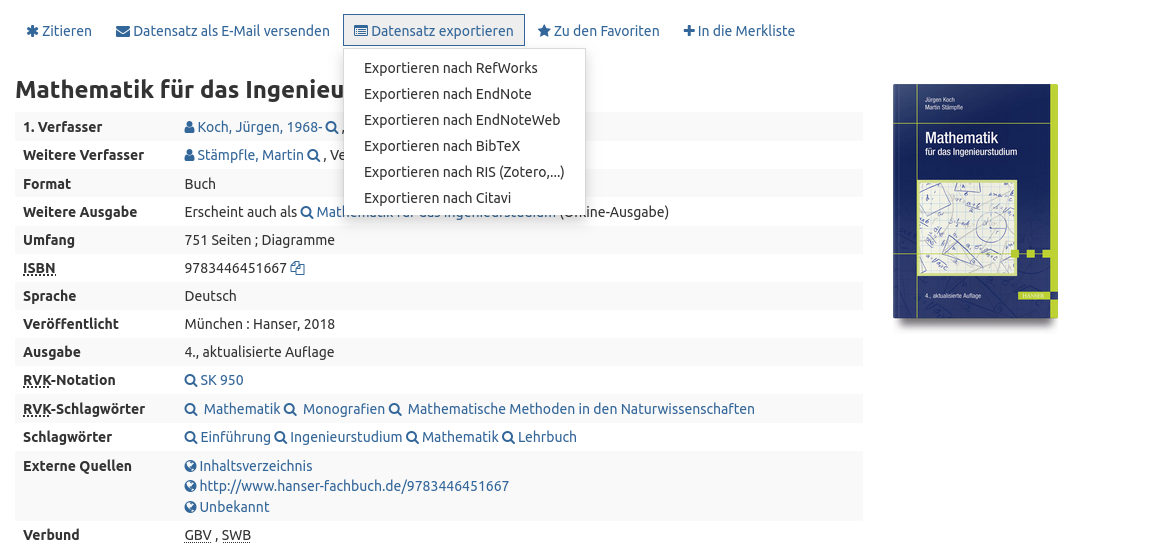
\includegraphics[width=.8\textwidth]{graphics/boss}}
      \only<2>{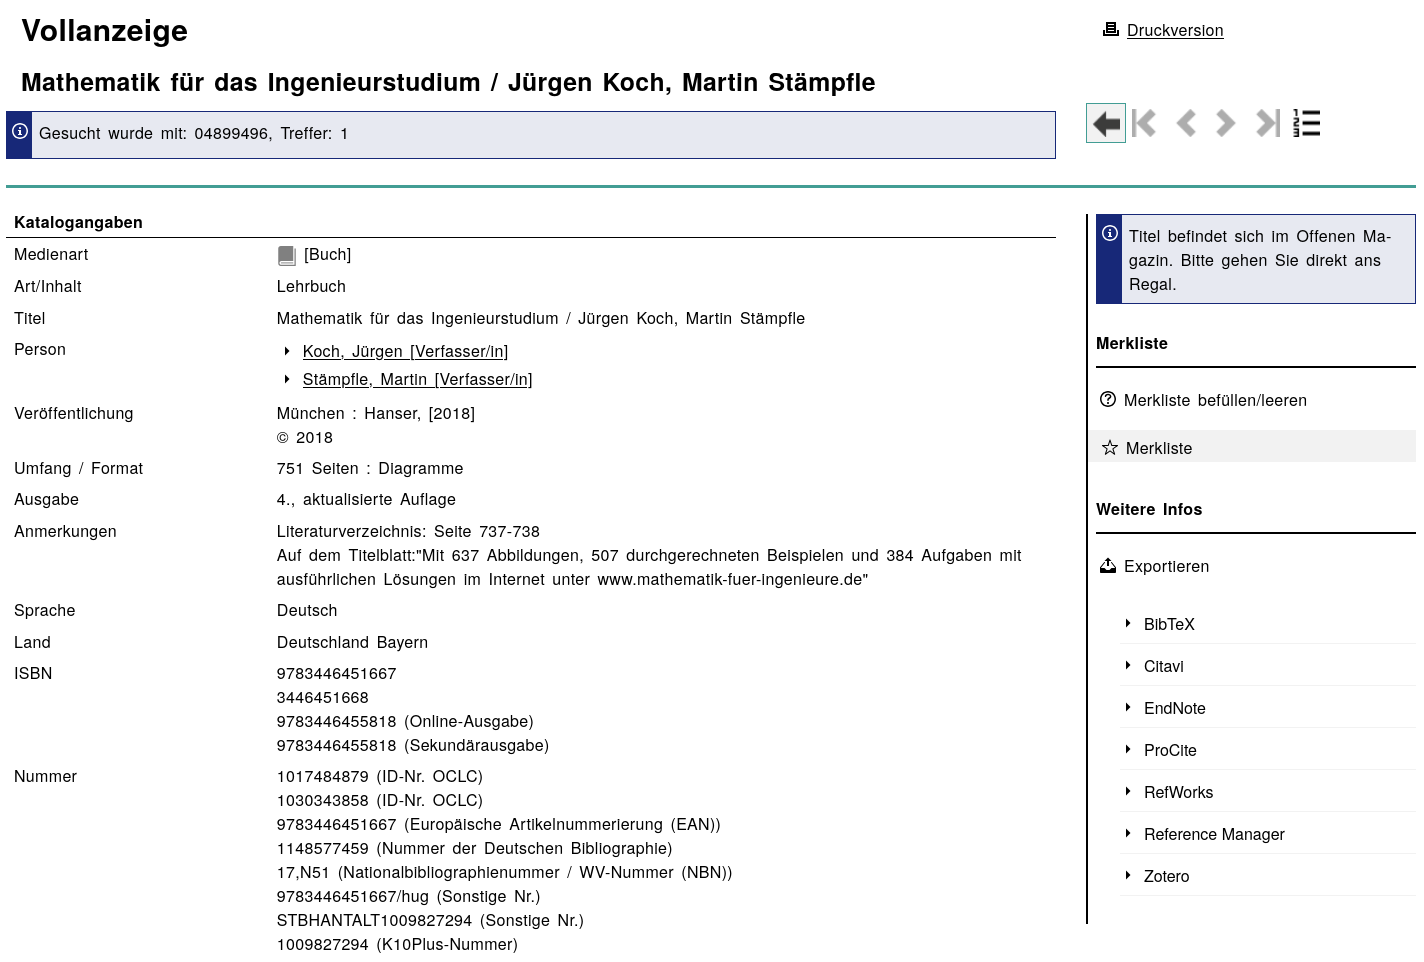
\includegraphics[width=.7\textwidth]{graphics/blb}}
    \only<3->{\item Verlage\\}
      \only<4>{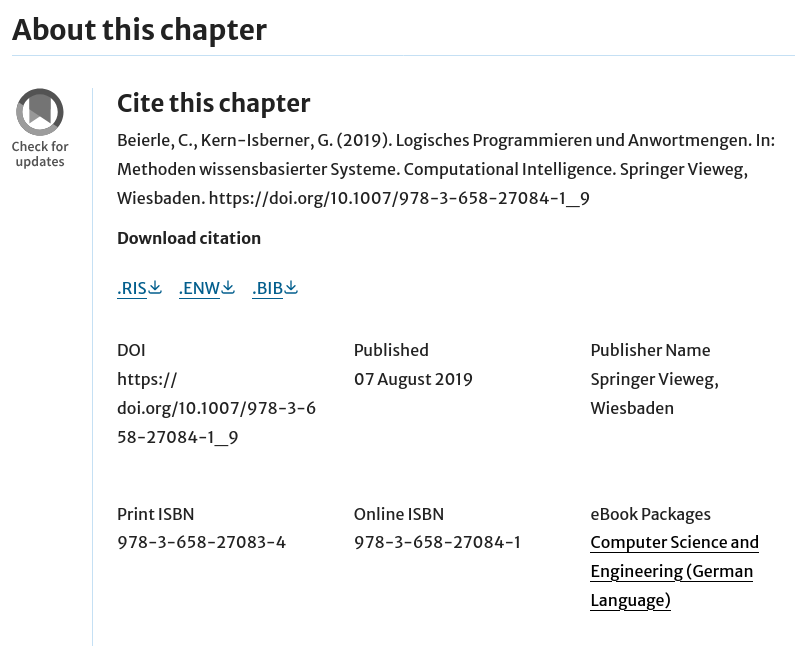
\includegraphics[width=.6\textwidth]{graphics/springer}}
      \only<5>{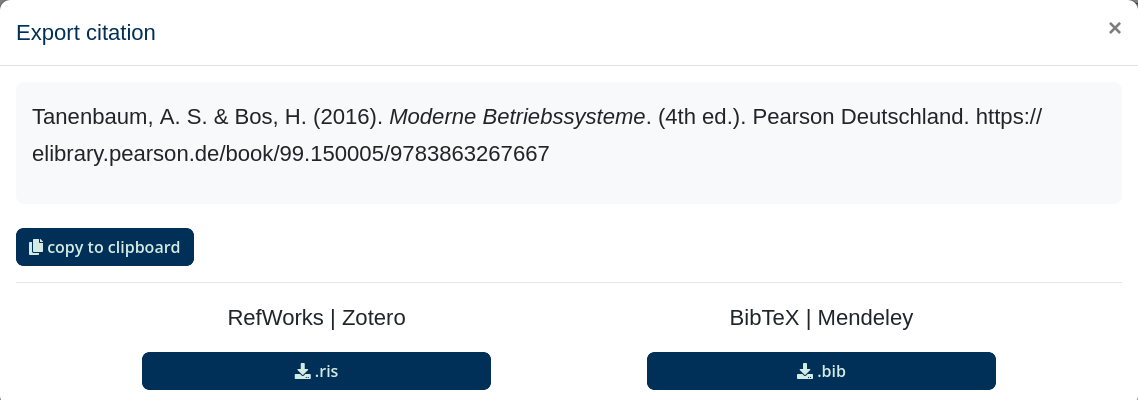
\includegraphics[width=.7\textwidth]{graphics/pearson}}
    \only<6->{\item Literaturverwaltung}
  \end{itemize}
\end{frame}

\begin{frame}{Exkurs: Literaturverwaltung}
  \only<1>{\centering 
\includegraphics[width=.9\textwidth]{graphics/bibliothek}}
  \only<2->{
    \begin{itemize}
      \item Verschiedene Programme zur Literaturverwaltung verfügbar
        \begin{itemize}
          \item \href{https://www.zotero.org/}{Zotero} (Open-Source, Crossplattform)
          \item \href{https://lumivero.com/products/citavi/}{Citavi} (Keine Hochschullizenz mehr in Baden-Württemberg)
          \item \href{https://www.mendeley.com/}{Mendeley}
        \end{itemize}
      \item bieten Integrationen in WYSIWYG-Editoren
      \item können auch nach Bib\TeX{} exportieren
    \end{itemize}
  }
\end{frame}

\begin{frame}{Exkurs: Literaturverwaltung -- Zotero}
  \begin{itemize}
    \item guter automatischer Export mit \href{https://retorque.re/zotero-better-bibtex/}{Better Bib\TeX{} for Zotero}
    \item generiert automatisch Bib\TeX{} mit allen Literatureinträgen einer Sammlung
    \item hält Datei bei Änderungen oder neu hinzufügten Dateien aktuell
      \bigskip
    \item einfach neue Literatur in Zotero einfügen mit \href{https://www.zotero.org/download/}{Zotero Connector}
  \end{itemize}
\end{frame}

\begin{frame}{Literatur -- Meine Empfehlungen}
  \begin{itemize}
    \item Verschiedene Literaturarten (Bücher, Paper, Thesen, Webseiten) in verschiedenen Untersammlungen verwalten
    \item pro Untersammlung ein automatischer Bib\LaTeX{}-Export
    \item Bib\LaTeX{}-Dateien in einen eigenen Unterordner
  \end{itemize}
\end{frame}

\begin{frame}[fragile]{Einbinden der Literatur in das Dokument}
  \inputminted{latex}{codebeispiele/inclusion-literature.tex}
\end{frame}

\begin{frame}[fragile]{Zitieren im Text}
  \begin{itemize}
    \item Zitate werden mit \verb|\cite{<citation-key>}| getätigt
    \item \verb|\parencite{<citation-key>}| setzt um Zitat Klammern
    \item \verb|\citeauthor{<citation-key>}| zitiert Autor:innen
    \item \verb|\citetitle{<citation-key>}| zitiert Titel
      \bigskip
    \item Standardmäßig wird nur Literatur im Literaturverzeichnis ausgegeben, das auch im Text zitiert wurde
      \begin{itemize}
        \item \verb|\nocite{<citation-key>}| fügt ein unzitiertes Werk ins Literaturverzeichnis ein
        \item \verb|\nocite{*}| zeigt alle Werke im Literaturverzeichnis an
      \end{itemize}
  \end{itemize}
\end{frame}

\begin{frame}[fragile]{Zitationsstile}
  \begin{itemize}
    \item Harvard-Stil (mit \href{https://ctan.org/pkg/biblatex-iso690?lang=en}{ISO 690 Literaturverzeichnis}): Koch, 2018
      \begin{minted}{latex}
\usepackage[style=iso-authoryear,natbib=true,
            useauthor=true]{biblatex}
\DeclareNameAlias{default}{family-given/given-family}
      \end{minted}
    \item Alphabetisch: [Koc18]
      \begin{minted}{latex}
\usepackage[style=alphabetic]{biblatex}
      \end{minted}
    \item Draft (geeignet zum Debuggen): \verb|<citation-key>|
      \begin{minted}{latex}
\usepackage[style=draft]{biblatex}
      \end{minted}
  \end{itemize}
\end{frame}

\begin{frame}[fragile]{Kompilieren mit Literatur}
  \begin{itemize}
    \item Literaturverzeichnis muss separat verarbeitet werden
    \item daher folgende Befehlsausführung notwendig:
      \begin{itemize}
        \item \verb|pdflatex|
        \item \verb|biber|
        \item \verb|pdflatex|
        \item \verb|pdflatex|
      \end{itemize}
    \item Manche Editoren bieten diese Kette unter "pdf\LaTeX{} + Bib\LaTeX{} + pdf\LaTeX{} (2x)" oder ähnlichen Optionen an
  \end{itemize}
\end{frame}

\section{Dokumentformatierung}

\begin{frame}[fragile]{Formatierungsoptionen}
  \begin{itemize}
    \item Papierformat
      \begin{itemize}
        \item wird in den Optionen zur Dokumentenklasse gesetzt
        \item A4: \verb|a4paper|
        \item A5: \verb|a5paper|
        \item Letter: \verb|letterpaper|
      \end{itemize}
    \item Seitenränder
      \begin{itemize}
        \item Mit Geometry-Paket
          \inputminted{latex}{codebeispiele/geometry.tex}
      \end{itemize}
  \end{itemize}
\end{frame}

\begin{frame}[fragile]{Querformat}
  \begin{itemize}
    \item Gesamtes Dokument im Querformat
      \begin{minted}{latex}
\documentclass[a4paper,landscape]{...}
      \end{minted}
    \item Einzelne Seiten im Querformat (nützlich für große Tabellen oder breite Abbildungen)
      \inputminted{latex}{codebeispiele/landscape.tex}
  \end{itemize}
\end{frame}

\begin{frame}[fragile]{Header und Footer}
  \begin{itemize}
    \item Kopf- und Fußzeilen können mit \verb|scrlayer-scrpage| konfiguriert werden
    \item Dafür muss der Style \verb|\pagestyle{scrheadings}| genutzt werden
    \item Inhalt der Zeilen wird dann mit
      \begin{itemize}
        \item \verb|ihead| bzw. \verb|ifoot| (inner)
        \item \verb|chead| bzw. \verb|cfoot| (center)
        \item \verb|ohead| bzw. \verb|ofoot| (outer)
      \end{itemize}
      beschrieben
    \item Bei zweiseitigen Layouts ist \verb|outer| am Rand der Seite und \verb|inner| an der Buchfalz
    \item \verb|\pagemark| enthält die aktuelle Seite
    \item Mit \verb|\pagestyle{empty}| werden keine Kopf- und Fußzeilen angezeigt
  \end{itemize}
\end{frame}

\begin{frame}[fragile]{Header und Footer -- Beispiel}
  \inputminted{latex}{codebeispiele/header-footer.tex}
\end{frame}

\section{Externe Dateien}

\begin{frame}[fragile]{Externe Dateien einbinden -- SVG}
  \begin{itemize}
    \item Nicht nativ möglich -- \LaTeX{} nutzt für Vektorgraphiken PDF
    \item Pakete ermöglichen jedoch automatische Konvertierung
    \item Nutzt dafür Inkscape und ImageMagick (\verb|convert|)
    \item dafür ist wieder die Option \verb|-shell-escape| nötig!
    \inputminted{latex}{codebeispiele/include-svg.tex}
    \item Alternativ Vektordateien direkt als PDF bereitstellen und mit \verb|\includegraphics| einbinden
  \end{itemize}
\end{frame}

\begin{frame}[fragile]{Externe Dateien einbinden -- PDF}
  \begin{itemize}
    \item PDF-Dateien als ganze Seiten einfügen (bspw. externe Dokumente im Anhang)
      \only<1>{\inputminted[lastline=6]{latex}{codebeispiele/include-pdf.tex}}
      \only<2>{
    \item PDF zum Inhaltsverzeichnis hinzufügen
      \inputminted[firstline=8]{latex}{codebeispiele/include-pdf.tex}
    }
  \end{itemize}
\end{frame}

\subsection{\LaTeX{}-Dateien strukturieren}

\begin{frame}[fragile]{Modularisierung}
  \begin{itemize}
    \item Bei größeren Projekten (> 2 Seiten) nicht alles in einer Datei behalten
    \item \LaTeX{}-Dateien können mit \verb|\include{<filename>}| oder \verb|\input{<filename>}| eingebunden werden
      \begin{itemize}
        \item \verb|\include| für Kapitel/große Abschnitte -> fügt automatisch einen Seitenumbruch ein
        \item \verb|\input| für Unterkapitel/kleinere Abschnitte
      \end{itemize}
    \item eine Datei für jedes Kapitel und den eröffnenden Text, dann jedes Unterkapitel aus der eigenen Datei einbinden
  \end{itemize}
\end{frame}

\begin{frame}[fragile]{Beispielhafte Dateistruktur}
  \lstinputlisting{codebeispiele/example-filestructure.txt}
\end{frame}

\begin{frame}[fragile]{Hauptteile eines Dokuments}
  \inputminted{latex}{codebeispiele/parts-of-document.tex}
\end{frame}

\section{Ausblick}

\begin{frame}{Was kann \LaTeX{} noch?}
  \begin{itemize}
    \item Präsentationen
    \item Zeichnen mit TikZ
    \item Plotting mit pdfPlots
    \item Chemische Formeln mit chemfig
    \bigskip
    \item Mathesyntax in vielen anderen Programmen
  \end{itemize}
\end{frame}

\begin{frame}{Nächste Projekte für \LaTeX{}?}
  \begin{itemize}
    \item Wissenschaftliches Dokumentieren
    \item Praxissemesterbericht
    \item Thesis
    \bigskip
    \item Bewerbungsunterlagen
  \end{itemize}
\end{frame}

\begin{frame}[fragile]{Bewerbungsunterlagen}
  \begin{columns}
    \column{.5\textwidth}
      \centering
      \begin{itemize}
        \item Lebenslauf mit \verb|moderncv|
      \end{itemize}
      
\includegraphics[height=.7\textheight]{Lebenslauf}
    \column{.5\textwidth}
      \centering
      \begin{itemize}
        \item Anschreiben mit \verb|dinbrief|
      \end{itemize}
      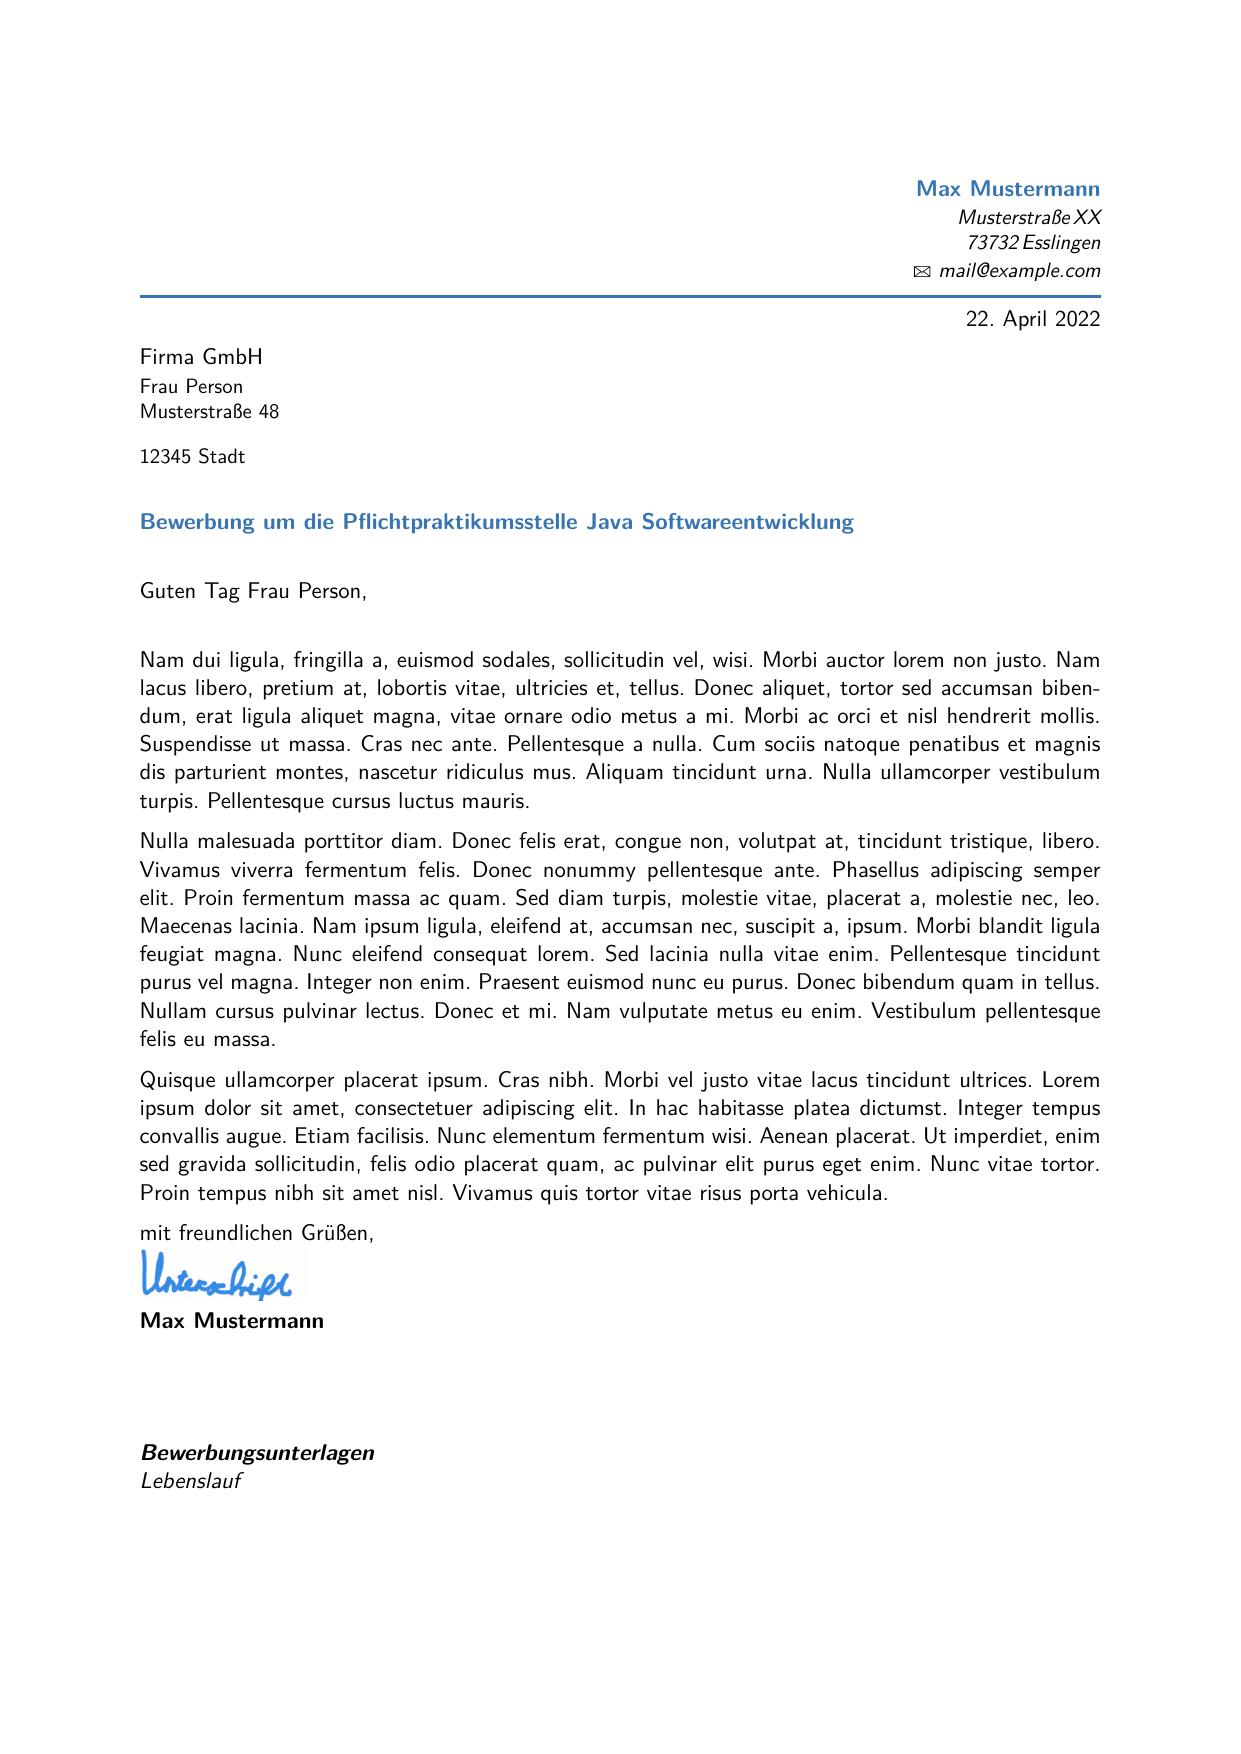
\includegraphics[height=.7\textheight]{Anschreiben}
  \end{columns}
\end{frame}

\begin{frame}[fragile]{Wohin bei Problemen?}
  \begin{itemize}
    \item \verb|texdoc <paketname>|
    \item Suchmaschine des Vertrauens
    \item \href{https://de.wikibooks.org/wiki/LaTeX-Kompendium}{\LaTeX-Kompendium}
    \item \href{https://www.overleaf.com/learn}{Overleaf documentation}
    \item \href{https://golatex.de/wiki/index.php/Hauptseite}{Go\LaTeX-Wiki}
    \item \href{https://tex.stackexchange.com}{\TeX-Stackexchange}
  \end{itemize}
\end{frame}

\maketitle

\end{document}
